\chapter{Herramientas para medir tolerancia a fallas enmascarante}
\label{cap:tool}

En este capítulo presentamos {\MaskD} y {\Tolerange}, dos herramientas automáticas diseñadas para medir el nivel de tolerancia a fallas entre componentes de software. 
%descritos por medio de un lenguaje de comandos con guardas.
Las herramientas se enfocan en medir componentes tolerantes a fallas de forma enmascarante, es decir, programas que enmascaran fallas de tal manera que no puedan ser observadas por el ambiente. La tolerancia a fallas enmascarante usualmente se clasifica como el el tipo de tolerancia mas beneficioso y es a su vez una propiedad altamente deseable para sistemas críticos. 
Las herramientas toman como entrada un modelo nominal y un modelo de su implementación tolerante a fallas, estos modelos son LTS y PTS en el caso de {\MaskD} y {\Tolerange}, respectivamente. {\MaskD} computa automáticamente la distancia de enmascaramiento entre estos modelos, mientras que {\Tolerange} computa el número esperado de hitos logrados por el modelo de implementación antes de entrar en un estado de falla.  

Estas herramientas están diseñadas para darle soporte a ingenieros de software en el análisis y diseño de sistemas tolerantes a fallas. 
Por lo tanto, los usuarios pueden comparar los resultados de las medidas entre distintas implementaciones y el modelo nominal, y así seleccionar la implementación que mejor se adapte a sus preferencias.
%En este capítulo se introducen herramientas originales destinadas a medir el nivel de masking-tolerancia de un modelo tolerante a fallas respecto a un modelo nominal. En particular se introducen dos componentes, {\MaskD} y {\Tolerange}, para la cuantificación del nivel de tolerancia a fallas de sistemas no estocásticos y estocásticos bajo la consideración de fallas, respectivamente.
Las herramientas presentadas en el presente capítulo implementan los algoritmos de los Capítulos~\ref{cap:maskingMeasure} y \ref{cap:maskProb}.

\section{MaskD} \label{sec:maskD}

\MaskD~es una herramienta de código abierto y libre  programa en \textsf{Java}, disponible en \cite{MaskD}. La herramienta  toma como entrada un modelo nominal y su implementación tolerante a fallas, y produce como salida la distancia de enmascaramiento entre ellos, la cual es un valor en el intervalo $[0,1]$.
Los modelos de entrada se describen utilizando el lenguaje de comandos con guardas introducido en \cite{AroraGouda93}, un lenguaje de programación simple para describir algoritmos tolerantes a fallas, que permite construcciones básicas de programas concurrentes.
Más precisamente, un programa descrito en este lenguaje es una colección de procesos, donde cada proceso está compuesto por una colección de acciones etiquetadas del estilo: $[\mathit{Label}]~\mathit{Guard} \rightarrow \mathit{Command}$, donde $\mathit{Guard}$ es una condición lógica sobre el estado actual del programa, $\mathit{Command}$ es una colección de asignaciones básicas que se ejecutan simultáneamente, y $\mathit{Label}$ es un nombre para la acción.
Estas construcciones sintácticas se denominan acciones. El lenguaje también permite a los usuarios etiquetar una acción como \emph{internal} (es decir, acciones silenciosas). Esto es importante para abstraerse de los mecanismos internos de el sistema que se modela y permitir construir modelos más complejos. Además, algunas acciones pueden ser etiquetadas como \emph{faulty} para indicar que representan fallas. La gramática completa para el lenguaje de modelado se encuentra en el apéndice~\ref{cap:appendix2}.
%
\begin{figure}[t]
\centering
\begin{minipage}[t]{.47\textwidth}
\fontsize{10}{10}\selectfont\ttfamily
\begin{tabbing}
x\=xxxxxxxx\=xxxxxxxxxxxx\=xx\=xxx\= \kill    
Process MEMORIA \{\\[1ex]
\>r : BOOL;  // valor observable \\ 
\>b0 : BOOL; // bit de memoria\\[1ex]
\>Initial: b0 \&\& r;\\[1ex]
%\>                   \>\>// 1 = refreshing\\[1ex]
\>[write1]  true -> b0=true, \\
\>\>~r=true; \\
\>[write0]  true -> b0=false, \\
\>\>~r=false; \\
\>[read0] !r -> r=r; // skip \\
\>[read1]  r -> r=r; // skip \\[1ex]
\}\\
\end{tabbing}
\end{minipage}
\caption{Modelo nominal para el ejemplo de la celda de memoria.} \label{fig:exam_1_mem_cell_nominal}
\end{figure}

\begin{figure}[t]
\centering
\begin{minipage}[t]{.47\textwidth}
\fontsize{10}{10}\selectfont\ttfamily
\begin{tabbing}
x\=xxxxxxxx\=xxxxxxxxxxxxx\=xxx\=xxx\= \kill    
Process MEMORIA\_FT \{\\[1ex]
\>r : BOOL; // valor observable \\
\>b0 : BOOL; // primer bit \\
\>b1 : BOOL; // segundo bit \\
\>b2 : BOOL; // tercer bit \\[1ex]
%\>\textcolor{red}{f : [0..1] init 0;} \>\>\textcolor{red}{// fault limiting artifact}\\[1ex]
\>Initial: b0 \&\& b1 \&\& b2 \&\& r;\\[1ex]
\>[write1]  true -> b0=true, b1=true,  \\
\>\>~b3=true, r=true; \>\> \\
\>[write0]  true -> b0=false, b1=false,  \\
\>\>~b3=false, r=false; \>\> \\
\>[read0]  !r -> r=r; // skip \\
\>[read1]  r ->  r=r; // skip \\
\>[fault1]  faulty true -> b0=!b0, r =(!b0\&\&b1)||(b1\&\&b2)|| \\ 
\>\>(!b0\&\&b2); // el primer bit falla  \\
\>[fault2]  faulty true -> b1=!b1, r =(b0\&\&!b1)||(!b1\&\&b2)|| \\ 
\>\>(b0\&\&b2); // el segundo bit falla  \\
\>[fault3]  faulty true -> b2=!b2, r =(b0\&\&b1)||(b1\&\&!b2)|| \\ 
\>\>(b0\&\&!b2); // el tercer bit falla  \\[1ex]
\}\\
\end{tabbing}
\end{minipage}
\caption{Modelo con fallas para el ejemplo de la celda de memoria.} \label{fig:exam_1_mem_cell_faulty}
\end{figure}

Como ejemplo, consideremos la celda de memoria vista en el Capítulo~\ref{cap:maskingMeasure}. 
Un estado en este sistema mantiene el valor corriente de la celda de memoria ($m=i$, para $i=0,1$), la operación de escritura permite cambiar este valor, y la operación de lectura retorna el valor almacenado.  
En este sistema, el resultado de una lectura dependerá del valor almacenado en la celda. 
Por lo tanto, una propiedad que uno podría asociar a este modelo es que el valor leído de la celda debe coincidir con el valor escrito por la última operación de escritura realizada por el sistema. 
    
Como se ha visto anteriormente, una falla potencial en este escenario ocurre cuando la celda pierde su carga de forma inesperada, y su valor almacenado cambia sin que se haya realizado una escritura (e.g., cambia de $1$ a $0$ por perdida de carga). Una técnica típica para lidiar con esta situación es el uso de \emph{redundancia}: 
en este caso, se utilizan tres bits de memoria en lugar de solo uno. Las operaciones de escritura son realizadas simultáneamente en los tres bits. 
La operación de lectura, por otro lado, retorna el valor que se repite al menos dos veces en los bits de memoria; esto se conoce como \emph{votación}. 
Las Figuras \ref{fig:exam_1_mem_cell_nominal} y \ref{fig:exam_1_mem_cell_faulty} muestran los procesos representando el modelo nominal y el modelo de la implementación tolerante a fallas, respectivamente, para este ejemplo. 

\subsection{Arquitectura de {\MaskD}}

\MaskD~es software de código abierto escrito en el lenguaje \textsf{Java}. La documentación y las instrucciones de instalación se pueden encontrar en \cite{MaskD}. La arquitectura de la herramienta se muestra en la Figura~\ref{fig:arch}.

\begin{figure}[ht]
    \centering
    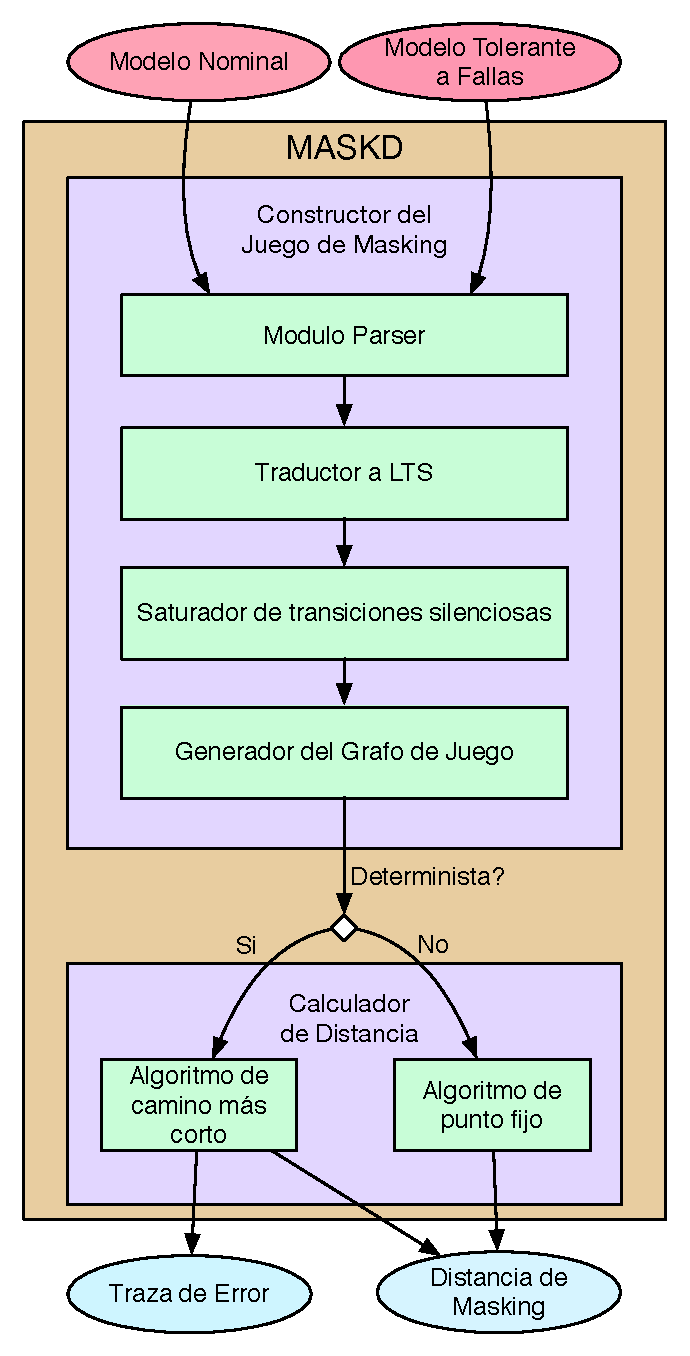
\includegraphics[scale=0.5]{Figs/MASKD_ARCH.pdf}
    \caption{Arquitectura de \textsf{MaskD}.}\label{fig:arch}
\end{figure}

    Discutiremos brevemente las componentes principales de la herramienta:
\begin{description}
    \item[Módulo Parser.] Realiza análisis sintáctico básico sobre los modelos de entrada y produce estructuras de datos que representan a  estas entradas. Para esto se utilizan las bibliotecas \textsf{Cup} y 
    \textsf{JFlex} para generar automáticamente el parser a partir de la gramática que describe el lenguaje de modelado.
    \item[Traducción a LTS.] Los modelos obtenidos del parser son traducidos a Sistemas de Transición Etiquetados (LTS), es decir, 
    grafos donde los vértices representan estados del programa y donde las transiciones mantienen información sobre las acciones de los modelos. 
    \item[Saturación de Transiciones Silenciosas.] Las transiciones internas/silenciosas en los LTS que representan los modelos de entrada son saturadas utilizando algoritmos estándar que provienen de teoría sobre álgebras de procesos \cite{Milner89}. Como resultado, se generan LTS saturados, estos son necesarios para verificar la relación de enmascaramiento cuando existen transiciones internas.
    \item[Generación del Grafo de Juego.] Utiliza los LTS saturados para producir un grafo de juego. Los nodos en este grafo codifican la configuración corriente del juego: 
    el próximo jugador que debe jugar, la última acción jugada, y referencias a los estados de los LTS de los modelos de entrada que se corresponden con la configuración actual del juego. 
    Las transiciones en este grafo corresponden a las posibles jugadas para los jugadores, es decir,  transiciones en los LTS originales.
    \item[Algoritmo de Camino más Corto.] Si los modelos de entrada son deterministas en las etiquetas de sus acciones, el algoritmo de camino más corto de Dial es utilizado para obtener el camino más corto hacia el estado de error, desde el cual se calcula el valor final.
    \item[Algoritmo de Punto Fijo.] Este es el algoritmo por defecto, funciona tanto para modelos deterministas como no deterministas en las etiquetas de sus acciones, utiliza una búsqueda de estilo bottom-up breadth-first para computar el valor del juego. 
    Este algoritmo se basa en algoritmos conocidos para resolver juegos de alcanzabilidad que utilizan conjuntos \emph{atractores} \cite{Jurd11}. 
    %This algorithm is polynomial in the game graph size.
\end{description}
Como se ha explicado más arriba, un punto interesante sobre la herramienta es que, para sistemas deterministas en sus acciones, la distancia de enmascaramiento entre dos sistemas puede ser computada recurriendo al algoritmo de camino más corto de Dial \cite{Dial69}, el cual tiene complejidad lineal con respecto al tamaño de los grafos utilizados para representar los sistemas.
En el caso de los sistemas no deterministas, se necesita un recorrido del estilo 
\textit{breadth-first search} con punto fijo, lo cual hace que el algoritmo sea menos eficiente. Sin embargo, incluso en este caso sigue siendo polinomial. 

%TODO: draw architecture and explain

%In order to measure the degree of masking fault-tolerance of a given system, 
%we start characterizing masking fault-tolerance via simulation relations between 
%two systems as defined in \cite{DemasiCMA17}. 
%The first one acting as a specification 
%of the intended behavior (es decir, nominal model) and the 
%second one as the fault-tolerant implementation (es decir, the extended model with 
%faulty behavior).
%The existence of a masking relation implies that the implementation masks the faults.
%Afterwards, we introduce a game characterization of 
%masking simulation and we enrich the resulting games 
%with quantitative objectives to define the notion of 
%\emph{masking fault-tolerance distance}, 
%where the possible values of the game belong to the interval $[0,1]$. 

\subsection{Modo de Uso}

El comando estándar para ejecutar {\MaskD} en un sistema operativo de estilo Unix es:
\\ 
\\
 \verb"./MaskD <options> <spec_path> <imp_path>"
\\
\\
En este caso la herramienta arroja como resultado la distancia de enmascaramiento entre la especificación y la implementación utilizando el algoritmo por defecto (algoritmo de punto fijo).
Algunos comandos opcionales incluyen: \verb"-t: print error trace", el cual muestra por salida estándar una traza hasta el estado de error bajo estrategias óptimas; y  \verb"-s: start simulation", el cual comienza una simulación manual desde el estado inicial.  
Obtener un camino hacia el estado de error es una funcionalidad útil para encontrar defectos en las descripciones de programas, los cuales pueden fallar por razones no intencionales. A su vez la traza sirve para ver como se comportan las estrategias óptimas de los jugadores. Una traza para el ejemplo de la celda de memoria se muestra en la Figura~\ref{fig:trace_mem_cell}. Los estados se muestran en el formato \verb"{spec_state, last_action_played, imp_state, player_turn}", donde \verb"spec_state" es el estado corriente del modelo nominal, \verb"last_action_played" es la última acción que se jugó (solo es relevante para estados del Verificador), \verb"imp_state" es el estado del modelo que representa a la implementación y \verb"player_turn" es el jugador cuyo turno corresponde jugar. En este caso, después de dos fallas (bits que cambian de valor sin que haya una escritura), al luego realizar una lectura, nos lleva al estado de error ya que en el modelo nominal el valor de la celda es $0$, mientras que el el modelo tolerante a fallas el valor leído en la mayoría (votación) de bits es $1$. Por otro lado, la funcionalidad de simulación permite al usuario seleccionar manualmente las acciones disponibles en cada punto del juego de enmascaramiento, lo cual también es útil para verificar que los modelos se comportan como el usuario espera.
Por defecto, \MaskD~computa la distancia de enmascaramiento para una entrada dada utilizando el algoritmo para sistemas no deterministas. 
El usuario puede utilizar la opción \verb"-det" para cambiar al algoritmo de distancia de enmascaramiento para sistemas deterministas.
\begin{figure}[t]
\centering
\begin{minipage}[t]{.47\textwidth}
\fontsize{10}{10}\selectfont\ttfamily
\begin{tabbing}
0. \{ <mr,mb0> , \# , <mr,mb0,mb1,mb2> , R \} \\ 
1. \{ <mr,mb0> , I\_m.fault1 , <mr,mb1,mb2> , V \} \\ 
2. \{ <mr,mb0> , \# , <mr,mb1,mb2> , R \} \\ 
3. \{ <mr,mb0> , I\_m.fault2 , <mb2> , V \} \\ 
4. \{ <mr,mb0> , \# , <mb2> , R \} \\ 
5. \{ <mr,mb0> , S\_m.read1 , <mb2> , V \} \\ 
6. ERR\_STATE \\ 
\end{tabbing}
\end{minipage}
\caption{Traza de Error para el ejemplo de la celda de memoria.} \label{fig:trace_mem_cell}
\end{figure}
\section{Tolerange} \label{sec:tolerange}

\Tolerange~toma como entrada también un modelo nominal y su implementación tolerante a fallas, esta vez siendo sistemas estocásticos, 
y produce como salida el número esperado de hitos acumulados que la implementación es capaz de preservar bajo un conjunto de fallas consideradas, esto es un valor en el intervalo $[0,\infty)$. Para asegurar que este valor está bien definido debemos asumir que la probabilidad de que el sistema eventualmente entre a un estado de falla es $1$. También asumimos que el ambiente juega de manera strong fair (si una acción o falla está habilitada con infinita frecuencia, entonces va a ocurrir con infinita frecuencia). A este tipo de sistemas los denominamos \emph{almost-surely failing bajo fairness} en el capítulo anterior. La herramienta puede verificar automáticamente si el juego derivado de los modelos es de este tipo.

Al igual que en {\MaskD}, un programa es una colección de procesos, donde cada uno está compuesto por una colección de acciones etiquetadas, esta vez de la forma: \verb"[Label]<reward>Guard->[P]Command++[Q]Command", donde: \verb"Guard" es una condición lógica sobre el estado actual del programa; \verb"Command" es 
una colección de asignaciones; \verb"Label" es el nombre de la acción; el entero positivo  \verb"reward" es 
opcional, y establece que la ejecución de esta acción cuenta como un ``hito'' de valor \verb"reward"; y \verb"++" es el operador de elección probabilista (aquí \verb"P" y \verb"Q" son las probabilidades correspondientes a cada rama de la elección; pueden haber varias ramas, siempre y cuando la suma de sus probabilidades sea $1$).
Al igual que antes, el lenguaje permite etiquetar a las acciones como \verb"faulty" para indicar que representan fallas. La gramática completa para el lenguaje de modelado se encuentra en el Apéndice~\ref{cap:appendix2}.

\iffalse
Para poder computar el número esperado de hitos logrados por la implementación, la herramienta utiliza nociones que vienen de la teoría de juegos.
More precisely,  first, we define a stochastic masking simulation game for any given nominal and fault-tolerant implementation model.
The basis of the game is similar to a probabilistic bisimulation game \cite{Stirling98}, and it is played by two players, 
named for convenience the Refuter ($\Refuter$) and the Verifier ($\Verifier$). The Verifier 
wants to prove that $s$ (a state of the specification) and $t$ (a state of the implementation) are \emph{probabilistic masking similar}, 
and the Refuter intends to disprove that.
The game starts from the pair of states $(s, t)$ and the following steps are repeated:
\begin{enumerate}
\item[1)] $\Refuter$ chooses either an action in the nominal model or an action in the implementation,  these actions have associated a probabilistic distribution,  which selects a next game state with certain probability.
Note that $\Refuter$ may select a fault.   Let $(a,\mu)$ be the action and distribution selected by $\Refuter$,
%  $\Refuter$ chooses either a transition $s \xrightarrow{a} \mu$ from
%  the nominal model or a transition $s' \xrightarrow{a} \mu'$ from the
%  implementation;
\item[2a)] If $a$ is not a fault,  $\Verifier$ has to match this with an action and a corresponding probabilistic distribution in the opposite model (say $(a,\mu')$),
it also selects a weighting function \cite{JonssonLarsen91} for $(\mu, \mu')$ (a function stating how the probabilities of both distributions are related).
\item[2b)]
  If $a$ is a fault,  $\Verifier$ can only select the Dirac
  distribution,  which gives probability $1$ to select as next state the actual state,   she also chooses the unique weighting function for
  $(\mu, \Dirac_{s})$. Intuitively, if  a fault occurs,  $\Verifier$ is obliged to mask the fault and cannot freely move in the nominal model.
\item[3)]
  The successor pair of states $(s',  t')$ is chosen  using the probabilities of the weighting function selected by $\Verifier$.
%% \item[1)] $\Refuter$ chooses action $a$ and distribution $\mu$ (resp. $\mu'$) such that $s \xrightarrow{a} \mu$ 
%% 		(resp. $s' \xrightarrow{a} \mu'$);
%% \item[2a)] If $a \notin \faults$, $\Verifier$ chooses a matching action $a$ and distribution $\mu'$ (resp. $\mu$) and 
%% 		a coupling $w$ such that $s' \xrightarrow{a} \mu'$ (resp. $s \xrightarrow{a} \mu$) and $w$ is coupling for $(\mu, \mu')$;
%% \item[2b)] If $a \in \faults$, $\Verifier$ selects the Dirac distribution  $\Dirac_{s}$ and a coupling $w$, such that 
%% 		$w$ is coupling for  $(\Dirac_{s}, \mu')$;
%% \item[3)] The successor pair of states $(t, t')$ is chosen probabilistically according to $w$.
\end{enumerate}
%
If the play continues forever, then the Verifier wins; otherwise, the
Refuter wins. %(Notice, in particular, that the Verifier loses if she cannot match a transition label, since choosing an arbitrary coupling is always possible.) Step 2b is the only one that differs from the usual
%bisimulation game.  This is needed because of the asymmetry produced by the
%transitions labeled with  faults. 
%Intuitively,  if the Refuter
%chooses to play a fault in the implementation, then the Verifier ought to
%mask the fault,  and she cannot freely move in the
%nominal model.  Summing up, the probabilistic step of a fault can only be
%matched by a Dirac distribution on the corresponding state of the specification. 

As explained above, we focus on those games
in which the refuter has probability $1$ of winning. Intuitively, this means that the system eventually will enter in an error state.  Furthermore, transitions could have associated a reward,  thus we obtain a quantitative version of these games: the Refuter intends to minimize the number of rewards collected by the Verifier, whereas the latter tries to maximize this number. Rewards are used to indicate the milestones that one  is interested in measuring. For instance, the number of ticks (discrete time) until the system fails.
\fi
%Accordingly, a bigger distance remarkably decreases fault-tolerance.
%We impleintroduce a game characterization of 
%masking simulation and we enrich the resulting games 
%with quantitative objectives to define the notion of 
%\emph{masking fault-tolerance distance}, 
%we start characterizing masking fault-tolerance via simulation relations between 
%two systems as defined in \cite{DemasiCMA17}. The first one acting as a specification 
%of the intended behavior (es decir, nominal model) and the 
%second one as the fault-tolerant implementation (es decir, the extended model with 
%faulty behavior).
%The existence of a masking relation implies that the implementation masks the faults.
%Afterwards, we introduce a game characterization of 
%masking simulation and we enrich the resulting games 
%with quantitative objectives to define the notion of 
%\emph{masking fault-tolerance distance}, 
%where the possible values of the game belong to the interval $[0,1]$. 
%In this game, the goal of the implementation is to mimic the behavior of the nominal model as much as possible.  In contrast, the
%nominal model tries to reach an error state as soon as possible. 
%Rewards are added to certain transitions in the game to reflect the fact that a fault was masked. 
%Thus, given a play (a maximal path in the game graph) a function $f_{\text{mask}}$ computes the value of the play: if it reaches the error state, the value is inversely proportional to the number of faults masked by the implementation; if the play is infinite,  it receives a value of $1$ indicating that the implementation was able to mask all the faults in the path. 
%The fault-tolerant implementation is masking fault-tolerant if the value of the game is $0$. Furthermore, the bigger the number, 
%the farther the masking distance between the fault-tolerant implementation and the specification. Accordingly, a bigger distance remarkably decreases fault-tolerance.
%Summing up,  as the final value gets closer to $1$ the implementation provides more masking fault-tolerance. 
%This value allows one to define a directed semi-metric, es decir, a function valuated in the interval $[0,1]$ that is transitive and it holds the triangle inequality, see \cite{CastroDDP18b} for the technical details.  
%The final value is given by the best play for the implementation given that the system uses an optimal play too.

\begin{figure}[t]
\centering
\begin{minipage}[t]{.47\textwidth}
\fontsize{10}{10}\selectfont\ttfamily
\begin{tabbing}
x\=xxxxxxxx\=xxxxxxxx\=xx\=xxx\= \kill    
Process NOMINAL \{\\[1ex]
\>v : INT; \\
\>s : INT;  		 \>\>// 0 = normal,\\ 
\>                   \>\>// 1 = refresh\\[1ex]
\>Initial: v==0 \&\& s==0;\\[1ex]
\>[write0]  !(s==1) -> v=0,s=0; \\
\>[write1]  !(s==1) -> v=1,s=0; \\[1ex]
\>[read0] !(s==1) \&\& v==0 -> v=v; \\
\>[read1] !(s==1) \&\& v==1 -> v=v; \\[1ex]
\>[tick] <1> s==0 -> 0.05 : s=1 \\
\>             \>\>++ 0.95 : v=v; \\[1ex]
\>[refresh] s==1 \&\& v==0 -> s=0, v=0; \\
\>[refresh] s==1 \&\& v==1 -> s=0, v=1; \\[1ex]
\}\\
\end{tabbing}
\end{minipage}
\caption{Modelo nominal para el ejemplo de la celda de memoria con refrescado.} \label{fig:exam_1_mem_cell_nom}
\vspace{-0.5cm}
\end{figure}

\begin{figure}[t]
\centering
\begin{minipage}[t]{.47\textwidth}
\fontsize{10}{10}\selectfont\ttfamily
\begin{tabbing}
x\=xxxxxxxx\=xxxxxxxx\=xx\=xxx\= \kill    
Process FAULTY \{\\[1ex]
\>v : INT; \\
\>s : INT;  		 \>\>// 0 = normal, 1 = refresh\\ 
\>                   \>\>// 2 = faulty\\[1ex]
\>Initial: v==0 \&\& s==0;\\[1ex]
\>[write0]  !(s==1) -> v=0,s=0; \\
\>[write1]  !(s==1) -> v=3,s=0; \\[1ex]
\>[read0] !(s==1) \&\& v<=1 -> v=v; \\
\>[read1] !(s==1) \&\& v>1 -> v=v; \\[1ex]
\>[tick] <1> s==0 -> 0.05 : s=1 \\
\>             \>\>++ 0.1 : s=2 \\
\>             \>\>++ 0.85 : v=v; \\
\>[tick] <1> s==2 -> 0.05 : s=1 \\
\>             \>\>++ 0.95 : v=v; \\[1ex]
\>[refresh] s==1 \&\& v<=0 -> s=0, v=0; \\
\>[refresh] s==1 \&\& v>1 -> s=0, v=3; \\[1ex]
\>[f] faulty s==2 \&\& v<3 -> s=0, v=v+1; \\
\>[f] faulty s==2 \&\& v>=3 -> s=0, v=2; \\
\>[f] faulty s==2 \&\& v>0 -> s=0, v=v-1; \\
\>[f] faulty s==2 \&\& v<=0 -> s=0, v=1; \\[1ex]
\}\\
\end{tabbing}
\end{minipage}
\vspace{-0.5cm}
\caption{Modelo de una implementación tolerante a fallas para el ejemplo de la celda de memoria con refrescado.} \label{fig:exam_1_mem_cell_ft}
\vspace{-0.5cm}
\end{figure}

Consideremos el ejemplo de la celda de memoria del Capítulo~\ref{cap:maskProb}. 
Las Figuras~\ref{fig:exam_1_mem_cell_nom} y  \ref{fig:exam_1_mem_cell_ft} muestran los procesos que representan al modelo nominal y la implementación tolerante a fallas, respectivamente. 
Las acciones $\texttt{read}i$
y $\texttt{write}i$ (para $i=0,1$) representan las acciones de lectura y escritura para el valor $i$.  El bit almacenado en la memoria está guardado en la variable~\texttt{v}.  La acción \texttt{tick} marca el paso de una unidad de tiempo y, con probabilidad \texttt{0.05}, habilita una acción de refrescado \texttt{refresh}). La variable \texttt{s}
indica si el sistema está en modo lectura/escritura, o produciendo un refrescado.
Una falla potencial en este escenario ocurre cuando una celda cambia de valor inesperadamente (e.g., como consecuencia de una interferencia electromagnética).
En la práctica, la ocurrencia de tal error tiene una cierta probabilidad. Nuevamente usamos  \emph{redundancia} para lidiar con estas fallas, %for instance
e.g., utilizando tres bits en lugar de uno. Luego, las operaciones de escritura se ejecutan simultáneamente sobre los tres bits mientras que una lectura retorna el valor de la mayoría.
El modelo de la Figura~\ref{fig:exam_1_mem_cell_ft} modela una implementación con triple redundancia y con las fallas mencionadas.  Ahora la variable \texttt{v} cuenta la cantidad de votos para el valor 1. Además de habilitar la acción de refrescado, un \texttt{tick} también puede habilitar la ocurrencia de una falla con probabilidad \texttt{0.1}.
%
La variable \texttt{s} ahora agrega un estado donde  puede ocurrir una falla ($\texttt{s}=2$).

\subsection{Arquitectura}
{\Tolerange} es un software de código abierto escrito en \textsf{Java}. 
%Documentation and installation instructions can be found at \cite{MaskD}. 
La arquitectura de la herramienta se muestra en la Figura~\ref{fig:arch_tolerange}.
\begin{figure}[ht]
    \centering
    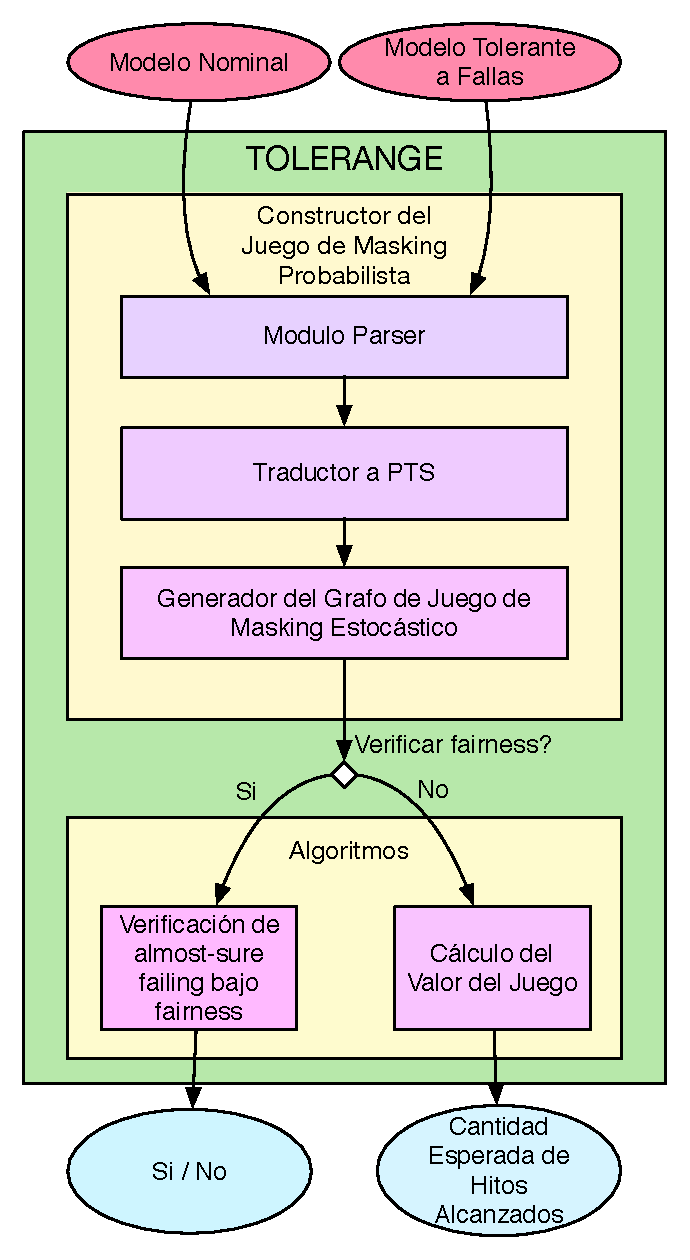
\includegraphics[scale=0.5]{Figs/TOLERANGE_ARCH.pdf}
    %\vspace{-0.4cm}
    \caption{Arquitectura de  \textsf{\Tolerange}.}\label{fig:arch_tolerange}
    %\vspace{-0.5cm}
\end{figure}
    En lo siguiente, describimos brevemente los componentes de la herramienta:
\begin{description}
    \item[Módulo Parser.] Realiza análisis sintáctico sobre los modelos de entrada, y produce estructuras de datos describiendo las entradas. Utiliza las librerías \textsf{Cup} y \textsf{JFlex}.
    \item[Traducción a PTS.] Los modelos obtenidos del parser se traducidos a Sistemas de Transición Probabilistas. 
    \item[Generación del Juego de Enmascaramiento Estocástico.] Se genera un juego de enmascaramiento estocástico para los PTS dados, donde las funciones de peso están capturadas simbólicamente a través de sistemas de ecuaciones (programación lineal).
    \item[Verificación de Terminación Bajo Fairness.] Se provee un algoritmo para verificar si un juego es casi-seguro terminante bajo fairness, consiste en computar los conjuntos predecesores en el grafo de juego simbólico. 
    \item[Cálculo del Valor del Juego (Algoritmo de Value Iteration).] El valor del juego puede ser computado solucionando una colección de ecuaciones funcionales a través de un algoritmo de \textit{value iteration}.
    Tomamos este valor como una medida de tolerancia a fallas.
    %This algorithm is polynomial in the game graph size.
\end{description}
\subsection{Modo de Uso}

El comando estándar para ejecutar {\Tolerange} en un sistema operativo Unix es:
\\ 
\\
 \verb"./Tolerange <options> <spec_path> <imp_path>"
\\
\\
    En este caso, la herramienta retorna la cantidad acumulada esperada de hitos logrados por la implementación.
Los comandos opcionales son: \verb"-f", para verificar si el juego es almost-sure failing bajo fairness;  \verb"-gurobi", el cual habilita {\Gurobi} \cite{gurobi} en lugar de {\SSC} \cite{SSC} para la programación lineal; y \verb"b=N" para establecer una cota superior de N para el valor del juego.
    Por defecto,  {\Tolerange} computa el valor del juego para las entradas dadas utilizando {\SSC} y una cota superior del número real máximo representable en {\Java}. 







